% Unofficial University of Cambridge Poster Template
% https://github.com/andiac/gemini-cam
% a fork of https://github.com/anishathalye/gemini
% also refer to https://github.com/k4rtik/uchicago-poster

\documentclass[final]{beamer}

% ====================
% Packages
% ====================

\usepackage[T1]{fontenc}
\usepackage{lmodern}
\usepackage[size=custom,width=84.1,height=59.4,scale=0.6]{beamerposter}
\usetheme{gemini}
\usecolortheme{cam}
\usepackage{graphicx}
\usepackage{makecell}
\usepackage{booktabs}
\usepackage[numbers]{natbib}
\usepackage{tikz}
\usetikzlibrary{positioning}
\usepackage{etoolbox} % for \ifnumcomp
\usepackage{listofitems}
\tikzset{>=latex} % for LaTeX arrow head
\colorlet{myred}{red!80!black}
\colorlet{myblue}{blue!80!black}
\colorlet{mygreen}{green!60!black}
\colorlet{mydarkred}{myred!40!black}
\colorlet{mydarkblue}{myblue!40!black}
\colorlet{mydarkgreen}{mygreen!40!black}
\tikzstyle{node}=[very thick,circle,draw=myblue,minimum size=22,inner sep=0.5,outer sep=0.6]
\tikzstyle{connect}=[->,thick,mydarkblue,shorten >=1]
\tikzset{ % node styles, numbered for easy mapping with \nstyle
  node 1/.style={node,mydarkgreen,draw=mygreen,fill=mygreen!25},
  node 2/.style={node,mydarkblue,draw=myblue,fill=myblue!20},
  node 3/.style={node,mydarkred,draw=myred,fill=myred!20},
}
\def\nstyle{int(\lay<\Nnodlen?min(2,\lay):3)} % map layer number onto 1, 2, or 3
\usepackage{pgfplots}
\pgfplotsset{compat=1.14}
\usepackage{anyfontsize}

% ====================
% Lengths
% ====================

% If you have N columns, choose \sepwidth and \colwidth such that
% (N+1)*\sepwidth + N*\colwidth = \paperwidth
\newlength{\sepwidth}
\newlength{\colwidth}
\setlength{\sepwidth}{0.025\paperwidth}
\setlength{\colwidth}{0.3\paperwidth}

\newcommand{\separatorcolumn}{\begin{column}{\sepwidth}\end{column}}

% ====================
% Title
% ====================

\title{Learning to Cooperate: Reinforcement Learning in the Iterated Prisoners Dilemma}

\author{Jonah Gräfe}

% \institute[shortinst]{\inst{1} Some Institute \samelineand \inst{2} Another Institute}

% ====================
% Footer (optional)
% ====================

\footercontent{
  \href{https://github.com/Jonah-gr/Reinforcement-Learning-IPD}{https://github.com/Jonah-gr/Reinforcement-Learning-IPD} \hfill
  Advances in Intelligent Systems \hfill
  \href{jonah.graefe@study.hs-duesseldorf.de}{jonah.graefe@study.hs-duesseldorf.de}}
% (can be left out to remove footer)

% ====================
% Logo (optional)
% ====================

% use this to include logos on the left and/or right side of the header:
\logoright{
\includegraphics[height=7cm]{logos/qr.PNG}}
\logoleft{
\includegraphics[height=7cm]{logos/HSD.png}}

% ====================
% Body
% ====================

\begin{document}

\tikzset{%
  every neuron/.style={
    circle,
    draw,
    minimum size=1cm
  },
  neuron missing/.style={
    draw=none, 
    scale=4,
    text height=0.333cm,
    execute at begin node=\color{black}$\vdots$
  },
}


% Refer to https://github.com/k4rtik/uchicago-poster
% logo: https://www.cam.ac.uk/brand-resources/about-the-logo/logo-downloads
% \addtobeamertemplate{headline}{}
% {
%     \begin{tikzpicture}[remember picture,overlay]
%       \node [anchor=north west, inner sep=3cm] at ([xshift=0.0cm,yshift=1.0cm]current page.north west)
%       {
\includegraphics[height=4.5cm]{logos/HSD.png}}; 
%     \end{tikzpicture}
% }

\begin{frame}[t]
\begin{columns}[t]
\separatorcolumn

\begin{column}{\colwidth}

  \begin{exampleblock}{Das iterierte Gefangenendilemma}

    Das wiederholte Gefangenendilemma (Iterated Prisoner's Dilemma, IPD) ist ein klassisches Problem der Spieltheorie, 
    das die Spannung zwischen Kooperation und Wettbewerb in wiederholten Interaktionen modelliert. In jeder Runde entscheiden sich 
    zwei Spieler unabhängig voneinander entweder für die Kooperation (C) oder für die Defektion (D). Ihre Entscheidungen bestimmen 
    ihre Auszahlungen auf der Grundlage einer Auszahlungsmatrix:

    \begin{table}
      \centering
      \begin{tabular}{l r r }
        \toprule
        \textbf{Player A/B} & \textbf{Cooperate (C)} & \textbf{Defect (D)}\\
        \midrule
        \textbf{Cooperate (C)} & (3, 3) & (0, 5) \\
        \midrule
        \textbf{Defect (D)} & (5, 0) & (1, 1) \\
        \bottomrule
      \end{tabular}
      \caption{Auszahlungsmatrix}
    \end{table}

    % \begin{itemize}
    %   \item Bei gegenseitiger Kooperation (C, C) werden beide Spieler mäßig belohnt.
    %   \item Gegenseitige Defektion (D, D) führt zu minimalen Belohnungen für beide.
    %   \item Ein Spieler, der abtrünnig wird, während der andere kooperiert (D, C), erhält die höchste Belohnung, aber der kooperierende 
    %   Spieler geht leer aus.
    % \end{itemize}
  
    % In der iterierten Version stehen sich die Spieler wiederholt gegenüber, so dass sich die Strategien auf der Grundlage des Verlaufs 
    % der Aktionen des Gegners anpassen können. Diese Dynamik führt Konzepte wie Vertrauen, Vergeltung und Vergebung ein und macht das 
    % IPD zu einem überzeugenden Rahmen für die Untersuchung von Entscheidungsfindung, sozialem Verhalten und dem Entstehen von Kooperation.

  \end{exampleblock}

  
  \begin{block}{Basis-Strategien}
    \begin{table}
      \centering
      \begin{tabular}{l l}
        \toprule
        \textbf{Strategie} & \textbf{Beschreibung} \\
        \midrule
        Random & Entscheidet zufällig \\
        \midrule
        AlwaysCooperate & Kooperiert immer \\
        \midrule
        AlwaysDefect & Defektiert immer \\
        \midrule
        Provocative & Defektiert nach 2-mal kooperieren \\
        \midrule
        TitForTat & Imitiert den Gegner \\
        \midrule
        TitForTwoTats & Defektiert, wenn Gegner 2-mal defektiert \\
        \midrule
        TwoTitsForTat & Defektiert 2-mal, wenn Gegner defektiert \\
        \midrule
        TitForTatOppesite & Imitiert den Gegner gegenteilig \\
        \midrule
        Spiteful & Defektiert für immer, wenn Gegner defektiert \\
        \midrule
        GenerousTitForTat & Imitiert den Gegner aber vergibt zu 10\% \\
        \midrule
        Adaptive & \makecell{Defektiert, wenn Gegner >50\% in den letzten \\ 10 Runden defektiert hat} \\
        \midrule
        Pavlov & \makecell{Defektiert, wenn Entscheidungen in vorheriger \\ Runde unterschiedlich waren} \\
        \midrule
        Gradual & Defektiert genauso oft wie Gegner defektiert \\
        \midrule
        WinStayLoseShift & Ändert Strategie wenn reward < 1 \\
        \midrule
        SoftMajority & Defektiert, wenn Gegner >50\% defektiert \\
        \bottomrule
      \end{tabular}
    \end{table}
    Dazu kommen "Suspicious"-Strategien, als erstes defektieren. So kommt man auf insgesamt 24 Strategien.
  
  \end{block}
  

  \begin{block}{\(Deep\) Q-Learning}
    \textbf{Q-Learning-Agenten}
    \begin{enumerate}
      % \item \textbf{Zustände und Handlungen:} Die Umgebung ist in Zustände unterteilt, und für jeden Zustand kann der Agent eine Reihe 
      % von Aktionen ausführen.
      \item \textbf{Q-Werte:} Der Q-Wert stellt die erwartete kumulative Belohnung für das Ausführen einer Aktion in einem bestimmten 
      Zustand und das anschließende Befolgen der optimalen Strategie dar.
      \item \textbf{Aktualisierung:} \begin{equation*} Q(s, a)\leftarrow Q(s, a) + \alpha [r + \gamma \max_{a}Q(s', a) - Q(s, a)]
                                      \end{equation*}
            \begin{itemize}
              \item $s,a,s'$: Aktueller Zustand, durchgeführte Aktion und der nächste Zustand.
              \item $r$: Erhaltene Belohnung
              \item $\alpha$: Lernrate 
              \item $\gamma$ Diskontierungsfaktor
            \end{itemize}
      % \item \textbf{Exploration vs. Exploitation:} Der Agent wägt zwischen Exploration (Ausprobieren neuer Handlungen) und Exploitation 
      % (Nutzung bekannter Handlungen mit hohen Q-Werten) unter Verwendung einer Epsilon-Greedy-Strategie ab.
  \end{enumerate}

  \textbf{Deep Q-Learning-Agenten}

  \begin{enumerate}
    \item \textbf{Neuronales Netz:} Bildet Zustände auf Q-Werte für alle möglichen Aktionen ab. Dies ersetzt die Q-Tabelle.
    \item \textbf{Erfahrungswiedergabe:} Der Agent speichert vergangene Erfahrungen in einem Wiederholungspuffer.
    \item \textbf{Training}: Minimierung des MSE zwischen vorhergesagten Q-Werten und Ziel Q-Werten mit Hilfe Adam-Optimierers
  \end{enumerate}

%   \begin{figure}[h]
%     \centering
%     \begin{tikzpicture}[x=5cm,y=1.5cm]
%       \readlist\Nnod{4,5,3,2} % array of number of nodes per layer
%       \readlist\Nstr{20,64,2} % array of string number of nodes per layer
%       \readlist\Cstr{x,h^{(\prev)},y} % array of coefficient symbol per layer
%       \def\yshift{0.55} % shift last node for dots
      
%       % LOOP over LAYERS
%       \foreachitem \N \in \Nnod{
%         \def\lay{\Ncnt} % alias of index of current layer
%         \pgfmathsetmacro\prev{int(\Ncnt-1)} % number of previous layer
%         \foreach \i [evaluate={\c=int(\i==\N); \y=\N/2-\i-\c*\yshift;
%                      \x=\lay; \n=\nstyle;
%                      \index=(\i<\N?int(\i):"\Nstr[\n]");}] in {1,...,\N}{ % loop over nodes
%           % NODES
%           \node[node \n] (N\lay-\i) at (\x,\y) {$\strut\Cstr[\n]_{\index}$};
          
%           % CONNECTIONS
%           \ifnumcomp{\lay}{>}{1}{ % connect to previous layer
%             \foreach \j in {1,...,\Nnod[\prev]}{ % loop over nodes in previous layer
%               \draw[white,line width=1.2,shorten >=1] (N\prev-\j) -- (N\lay-\i);
%               \draw[connect] (N\prev-\j) -- (N\lay-\i);
%             }
%             \ifnum \lay=\Nnodlen
%               \draw[connect] (N\lay-\i) --++ (0.5,0); % arrows out
%             \fi
%           }{
%             \draw[connect] (0.5,\y) -- (N\lay-\i); % arrows in
%           }
          
%         }
%         \ifnum \lay<\Nnodlen
%           \path (N\lay-\N) --++ (0,1+\yshift) node[midway,scale=1.6] {$\vdots$}; % dots
%         \fi
  
%       }
      
%       % LABELS
%       \node[above=0.2,align=center,mydarkgreen] at (N1-1.90) {Input\\[-0.2em]layer};
%       \node[above=0.2,align=center,mydarkblue] at (N2-1.90) {Hidden\\[-0.2em]layer};
%       \node[above=0.2,align=center,mydarkblue] at (N3-1.90) {Hidden\\[-0.2em]layer};
%       \node[above=0.2,align=center,mydarkred] at (N\Nnodlen-1.90) {Output\\[-0.2em]layer};
      
%     \end{tikzpicture}
%     \caption{Q-Netzwerk mit $n$ Input, $64$ und $32$ Hidden und $2$ Output Neuronen.}
%     \end{figure}

\end{block}


  
  

\end{column}

\separatorcolumn

\begin{column}{\colwidth}

  
  \begin{block}{Q-Netzwerk}
    % \begin{center}
    \begin{figure}[h]
    \centering
    \begin{tikzpicture}[x=5cm,y=1.6cm]
      \readlist\Nnod{4,5,3,2} % array of number of nodes per layer
      \readlist\Nstr{20,64,2} % array of string number of nodes per layer
      \readlist\Cstr{x,h^{(\prev)},y} % array of coefficient symbol per layer
      \def\yshift{0.55} % shift last node for dots
      
      % LOOP over LAYERS
      \foreachitem \N \in \Nnod{
        \def\lay{\Ncnt} % alias of index of current layer
        \pgfmathsetmacro\prev{int(\Ncnt-1)} % number of previous layer
        \foreach \i [evaluate={\c=int(\i==\N); \y=\N/2-\i-\c*\yshift;
                     \x=\lay; \n=\nstyle;
                     \index=(\i<\N?int(\i):"\Nstr[\n]");}] in {1,...,\N}{ % loop over nodes
          % NODES
          \node[node \n] (N\lay-\i) at (\x,\y) {$\strut\Cstr[\n]_{\index}$};
          
          % CONNECTIONS
          \ifnumcomp{\lay}{>}{1}{ % connect to previous layer
            \foreach \j in {1,...,\Nnod[\prev]}{ % loop over nodes in previous layer
              \draw[white,line width=1.2,shorten >=1] (N\prev-\j) -- (N\lay-\i);
              \draw[connect] (N\prev-\j) -- (N\lay-\i);
            }
            \ifnum \lay=\Nnodlen
              \draw[connect] (N\lay-\i) --++ (0.5,0); % arrows out
            \fi
          }{
            \draw[connect] (0.5,\y) -- (N\lay-\i); % arrows in
          }
          
        }
        \ifnum \lay<\Nnodlen
          \path (N\lay-\N) --++ (0,1+\yshift) node[midway,scale=1.6] {$\vdots$}; % dots
        \fi
  
      }
      
      % LABELS
      \node[above=0.2,align=center,mydarkgreen] at (N1-1.90) {Input\\[-0.2em]layer};
      \node[above=0.2,align=center,mydarkblue] at (N2-1.90) {Hidden\\[-0.2em]layer};
      \node[above=0.2,align=center,mydarkblue] at (N3-1.90) {Hidden\\[-0.2em]layer};
      \node[above=0.2,align=center,mydarkred] at (N\Nnodlen-1.90) {Output\\[-0.2em]layer};
      
    \end{tikzpicture}
    \caption{Q-Netzwerk mit $n$ Input, $64$ und $32$ Hidden und $2$ Output Neuronen.}
    \end{figure}
    % \end{center}
    \end{block}


    % \begin{exampleblock}{Zufällige Entscheidungen}
    %   In folgenden Darstellungen (Figure 2-5) wurden 10000 Epochen, bestehend aus einem Spiel mit 100 Runden gegen eine zufällige aber 
    %   feste Reihenfolge von Basis-Strategien gespielt.
    %   \textbf{RandomAgent}
    %   \begin{figure}[h]
    %     \centering
    %     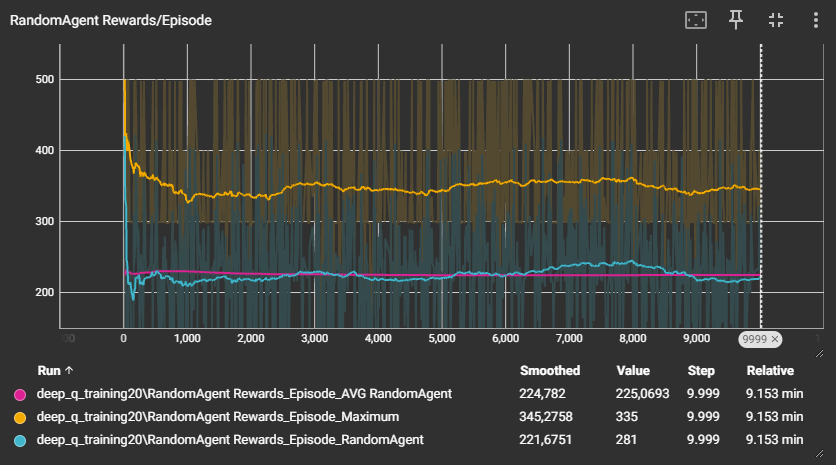
\includegraphics[width=20cm]{logos/random_agent.PNG}
    %     \caption{Geglättete Ergebnisse des RandomAgents. Pink: Durchschnittsbelohnung, Gelb: Maximum, Blau: Belohnung}
    %   \end{figure}
    % \end{exampleblock}
  
  \begin{block}{Zufällige Strategien}
    In folgenden Darstellungen (Figure 2-5) wurden 10000 Epochen, bestehend aus jeweils einem Spiel mit 100 Runden gegen eine zufällige aber 
    feste Reihenfolge von Basis-Strategien gespielt. \\
    \textbf{RandomStrategies}
    \begin{figure}[h]
      \centering
      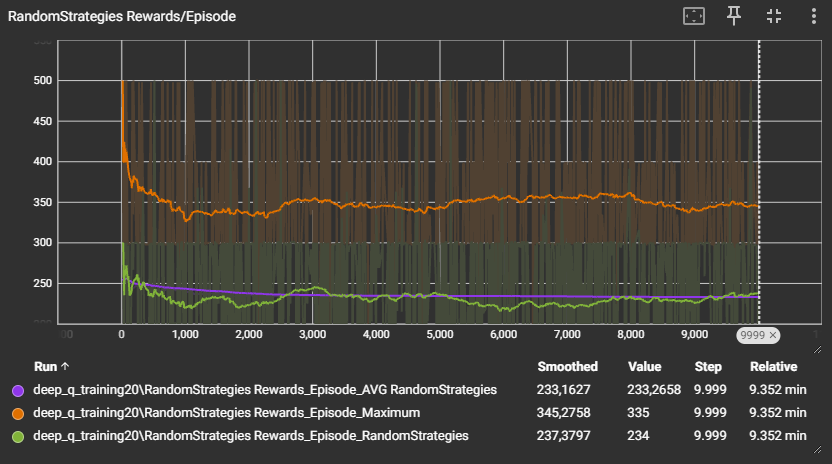
\includegraphics[width=20cm]{logos/random_strategies.PNG}
      \caption{Geglättete Ergebnisse der zufälligen Strategien. Lila: Durchschnittsbelohnung, Orange: Maximum, Grün: Belohnung}
    \end{figure}
  \end{block}


  \begin{alertblock}{Q-Learning Training}
    % In folgenden Darstellungen (Figure 2 und 3) wurden 10000 Epochen, bestehend aus einem Spiel mit 100 Runden gegen eine zufällige aber 
    % feste Reihenfolge von Basis-Strategien gespielt. \\
    \textbf{QLearningAgent} ($\alpha = 0.01$, $\gamma = 0.5$)
     \begin{equation*}
       Q = \left[ \begin{array}{cc} 6.0 & 3.99581385 \\ 7.99162798 & 4.22964461 \end{array} \right]
     \end{equation*}
    
     \begin{figure}[h]
      \centering
      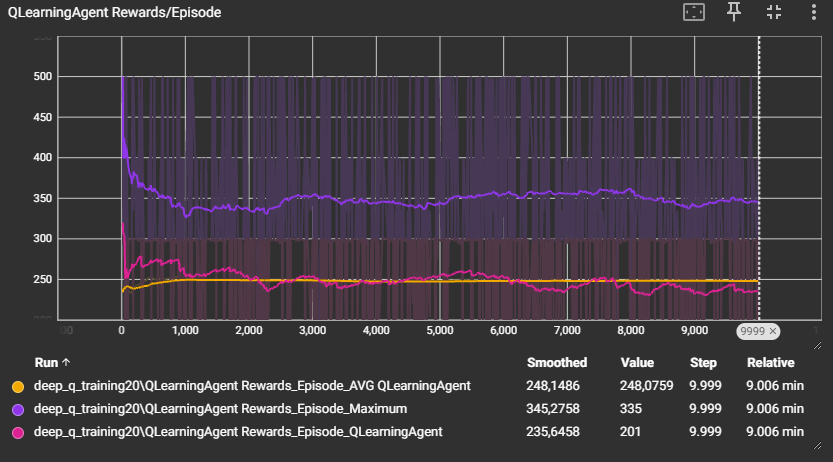
\includegraphics[width=20cm]{logos/qlearning.PNG}
      \caption{Geglättete Ergebnisse des QLearningAgents. Gelb: Durchschnittsbelohnung, Pink: Belohnung, Lila: Maximum}
    \end{figure}
  
  \end{alertblock}

  


\end{column}

\separatorcolumn

\begin{column}{\colwidth}

  \begin{alertblock}{Deep Q-Learning Training}
    \textbf{DeepQLearningAgent} ($\alpha = 0.001$, $\gamma = 0.99$)
    \begin{figure}[h]
      \centering
      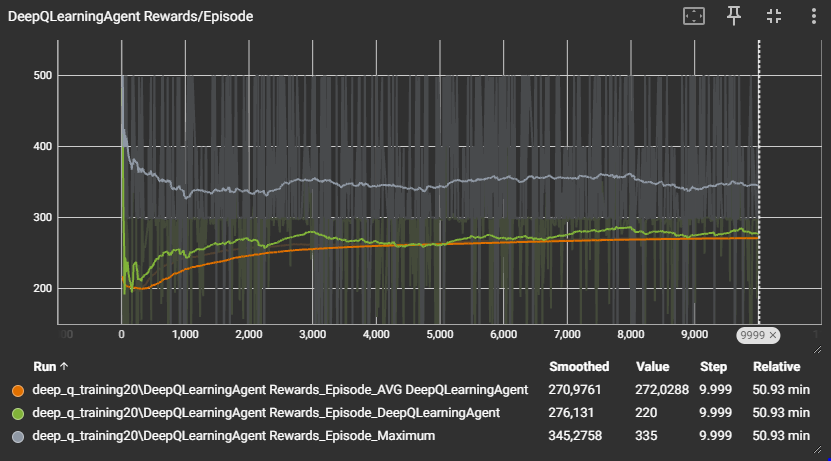
\includegraphics[width=20cm]{logos/deepq.PNG}
      \caption{Geglättete Ergebnisse des DeepQLearningAgents. Orange: Durchschnittsbelohnung, Grün: Belohnung, Grau: Maximum}
    \end{figure}

    \begin{figure}[h]
      \centering
      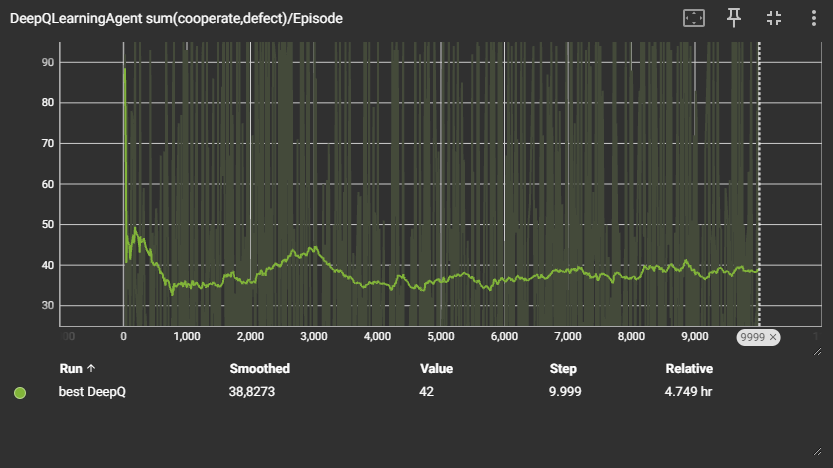
\includegraphics[width=20cm]{logos/co_de.PNG}
      \caption{Geglättete Summe von Kooperation ($0$) und Defektion ($1$) in jeder Epoche}
    \end{figure}
    
  \end{alertblock}

  \begin{alertblock}{Turnier-Ergebnisse}
    Jeder der folgenden Agenten hat in einem Turnier 100-Mal gegen jede Basis-Strategie gespielt:
     \begin{figure}[h]
      \centering
      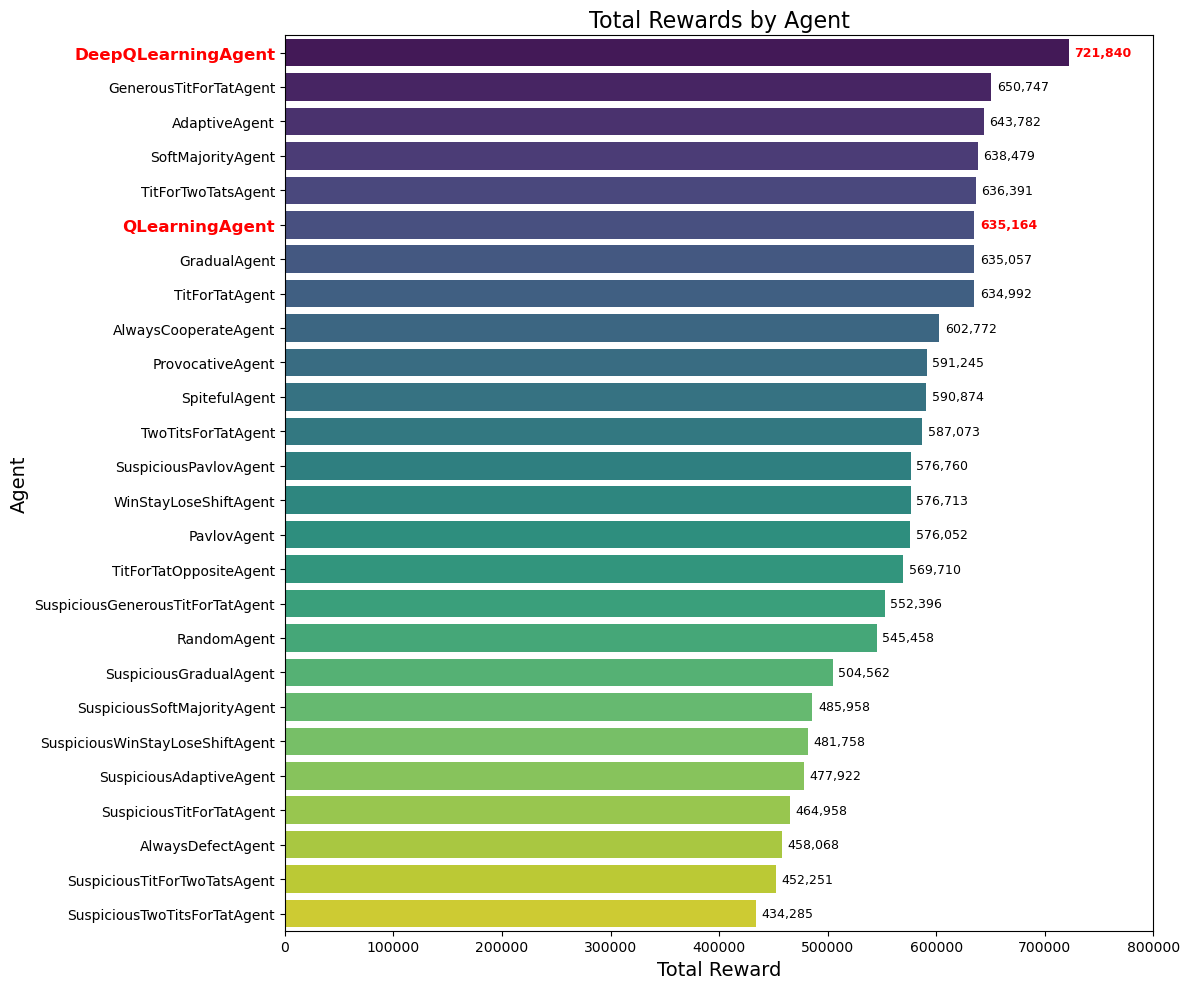
\includegraphics[width=20cm]{logos/tournament.png}
      \caption{Barplot der Gesamtbelohnungen aller Agenten}
    \end{figure}
  
  \end{alertblock}

\end{column}

\separatorcolumn
\end{columns}
\end{frame}

\end{document}
